\chapter{From Theory to Practice: Applications and Interventions}
\label{chap7}

Having established the theoretical foundations of the Random Voting Model and demonstrated its remarkable predictive power across diverse electoral contexts, we now turn our attention to practical applications. This chapter explores how our theoretical insights can be translated into concrete interventions that address two critical challenges facing modern democracies: increasing opinion polarization and concerns about electoral integrity. These applications represent the culmination of our scientific journey—where theoretical understanding transforms into tools for positive change.

\section{The Intervention Toolkit: Two Complementary Approaches}

Our research has developed two distinct but complementary tools for democratic intervention: the Random Nudge for reducing polarization in opinion dynamics, and the Random Voting Model as a statistical framework for analyzing electoral outcomes and detecting irregularities. Both approaches leverage randomness in different ways to understand and potentially improve democratic processes. The random nudge utilizes stochastic perturbations to break echo chambers and reduce polarization in opinion formation, while the RVM establishes statistical baselines against which electoral outcomes can be evaluated.

\section{Application 1: The Random Nudge for Depolarization}

As we explored in earlier chapters, opinion dynamics in complex social systems can lead to increasing polarization over time, with individuals becoming more extreme in their views and society segregating into opposed camps. Our random nudge strategy represents a novel intervention approach designed to counter these polarizing tendencies.

\subsection{The Mathematical Framework and Empirical Grounding}

The random nudge builds on a well-established model of opinion dynamics that incorporates homophily—the tendency of agents to connect with others holding similar opinions. This model successfully captures the formation of echo chambers and polarization observed in real social networks. In the model, N agents hold opinions $x_i$ on a continuous scale, where the sign of $x_i$ represents the agent's stance on an issue and $|x_i|$ represents their conviction.

The standard opinion dynamics are governed by:

\begin{equation}
    \dot{x}_i= -x_i + K \left(\sum^{N}_{j=1} A_{ij} (t)  \tanh{(\alpha x_j)}\right)
\end{equation}

where $K$ is the strength of social interaction, $\alpha$ is the controversialness of the issue, and $A_{ij}(t)$ is the temporal adjacency matrix determining which agents interact at time $t$. Crucially, the probability of interaction between agents is governed by homophily:

\begin{equation}
    P_{ij} = \frac{|x_i - x_j|^{-\beta}}{\sum_k{|x_i - x_k|^{-\beta}}}
\end{equation}

where $\beta$ is the homophily factor. When $\beta > 0$, agents with similar opinions are more likely to interact, leading to the formation of echo chambers and polarized states.

The random nudge intervention modifies this interaction probability as follows:

\begin{equation}
    \widetilde{P}_{ij} = p \times \frac{1}{N - 1} + (1 - p) \times P_{ij}
\end{equation}

where $p$ is the random nudge probability. With probability $p$, agents interact uniformly with any other agent (regardless of opinion similarity), and with probability $(1-p)$, they interact according to the homophily-based probability. This simple intervention introduces controlled randomness into the opinion formation process.

\subsection{Optimization for Maximum Depolarization}

The effectiveness of the random nudge depends on careful calibration of the nudge probability $p$. Our research shows that even small values of $p$ (around 0.01) can significantly reduce polarization. However, excessive randomness (high values of $p$) can lead to an undesirable effect called radicalization, where all agents converge to the same extreme stance.

We developed an optimization framework that balances depolarization against radicalization risk. Using multiple measures of polarization—including the distance between mean positive and negative opinions ($\bar{\Delta}$), the distance between peaks in bimodal distributions ($\Delta_{peak}$), and the standard deviation of the opinion distribution ($\sigma$)—we can identify the optimal nudge probability.

Our simulations demonstrate that all three measures of polarization decrease as a stretched exponential function $\exp(-p^\gamma)$ of the nudge strength, with $\gamma \approx 0.3$. However, the fraction of simulations leading to radicalization increases dramatically for $p > 10^{-2}$, creating a clear trade-off between depolarization and radicalization risk.

% \begin{figure}[h]
%     \centering
%     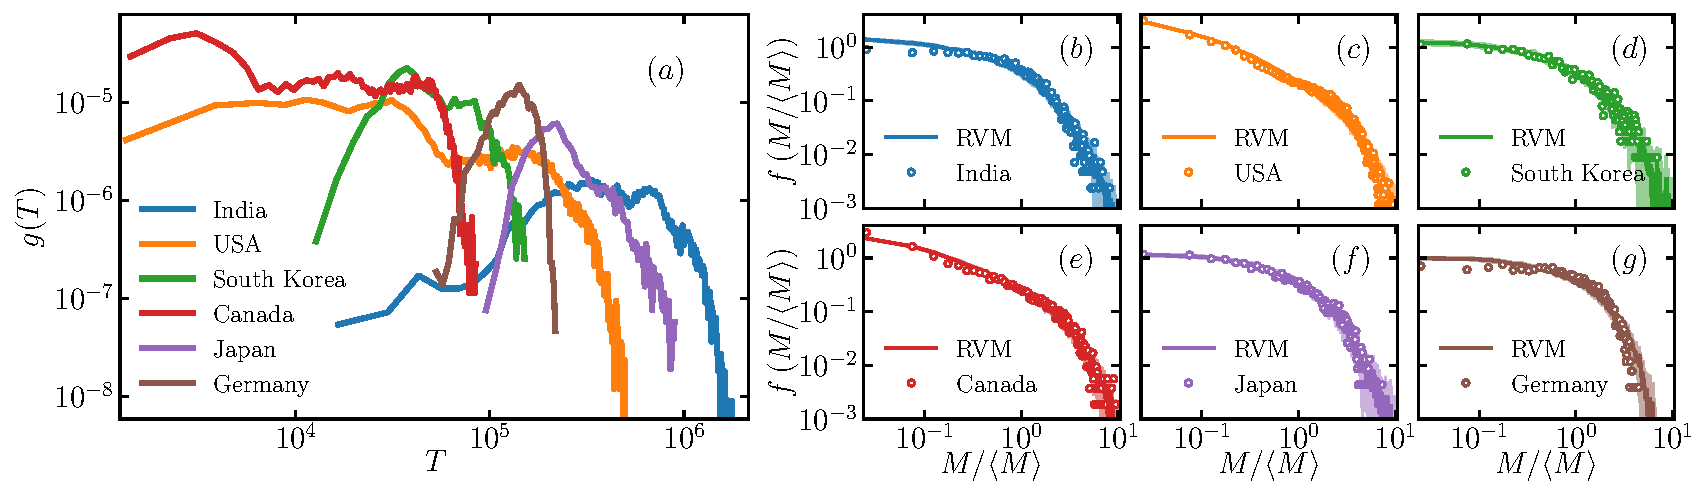
\includegraphics[width=0.8\linewidth]{chapters/chapter6/fig_1.pdf}
%     \caption{Impact of the random nudge on opinion distributions. Panel (a) shows the evolution of opinions without intervention, leading to polarized clusters. Panel (b) demonstrates how the optimized random nudge prevents cluster formation and maintains a more moderate distribution of opinions.}
%     \label{fig:randnudge}
% \end{figure}

\subsection{Network Effects and Echo Chamber Disruption}

The random nudge works by disrupting the formation of echo chambers in the social interaction network. Without the nudge, the network naturally segregates into distinct clusters of like-minded individuals, with few connections between opposing groups. This network structure reinforces polarization through repeated exposure to similar opinions.

When the random nudge is applied, the network becomes more integrated, with connections spanning across opinion divides. This structural change has profound effects on opinion dynamics. By exposing individuals to diverse viewpoints, the nudge prevents extreme opinions from being reinforced and allows moderate positions to persist.

Our analysis of the network structure reveals that without intervention, the average opinion of an agent's nearest neighbors strongly correlates with their own opinion—the signature of echo chambers. With the random nudge, this correlation weakens significantly, indicating successful disruption of echo chamber effects.

\subsection{Practical Implementation in Digital Platforms}

The random nudge can be implemented as an algorithmic intervention in social media recommendation systems and content delivery platforms. Rather than always showing users content that aligns with their existing views (which reinforces polarization), platforms could occasionally introduce content from diverse perspectives.

The practical implementation involves creating a latent space of content and user opinions, identifying users at risk of polarization, and introducing diverse content with appropriate frequency and intensity. This approach is non-invasive, as it does not require interpreting the specific opinions of users but simply introduces controlled randomness into the recommendation process.

For small enough values of the nudge probability, the platform remains engaging while maintaining sufficient diversity to prevent echo chambers. This balance is crucial for practical adoption, as interventions that significantly reduce user engagement are unlikely to be implemented by commercial platforms.

\subsection{Ethical Considerations and Limitations}

Any intervention in opinion formation processes raises important ethical questions about autonomy, manipulation, and transparency. The random nudge is designed to be transparent, with users aware that content diversity is being promoted; non-coercive, expanding exposure without forcing engagement; and balanced, avoiding both echo chambers and overwhelming users with contrary views.

The limitations of this approach include the challenge of accurately mapping opinion spaces, the potential for user disengagement, and varying effectiveness across different cultural and political contexts. Additionally, the random nudge cannot address structural causes of polarization such as economic inequality or institutional factors, and its effectiveness may be limited against deliberate disinformation campaigns.

\section{Application 2: The RVM as Diagnostic Tool}

While the Random Voting Model was initially developed to explain universal patterns in electoral statistics, it also provides a powerful diagnostic tool for evaluating electoral integrity. By establishing what electoral statistics should look like under fair competitive conditions, the RVM creates a baseline against which actual outcomes can be compared.

\subsection{From Universal Patterns to Anomaly Detection}

The RVM's prediction of universal patterns in the scaled specific margin distribution $F(x)$ provides an especially valuable diagnostic tool. As demonstrated in Chapter 5, this distribution follows a consistent pattern across 32 countries despite vast differences in their electoral systems, histories, and political cultures.

Significant deviations from this universal pattern may indicate unusual electoral dynamics that warrant further investigation. The RVM provides three specific diagnostic approaches: comparing a country's $F(x)$ distribution to the universal form, verifying that different electoral scales within a country show consistent statistical patterns, and tracking changes in electoral statistics over time to identify unusual shifts.

% \begin{figure}[h]
%     \centering
%     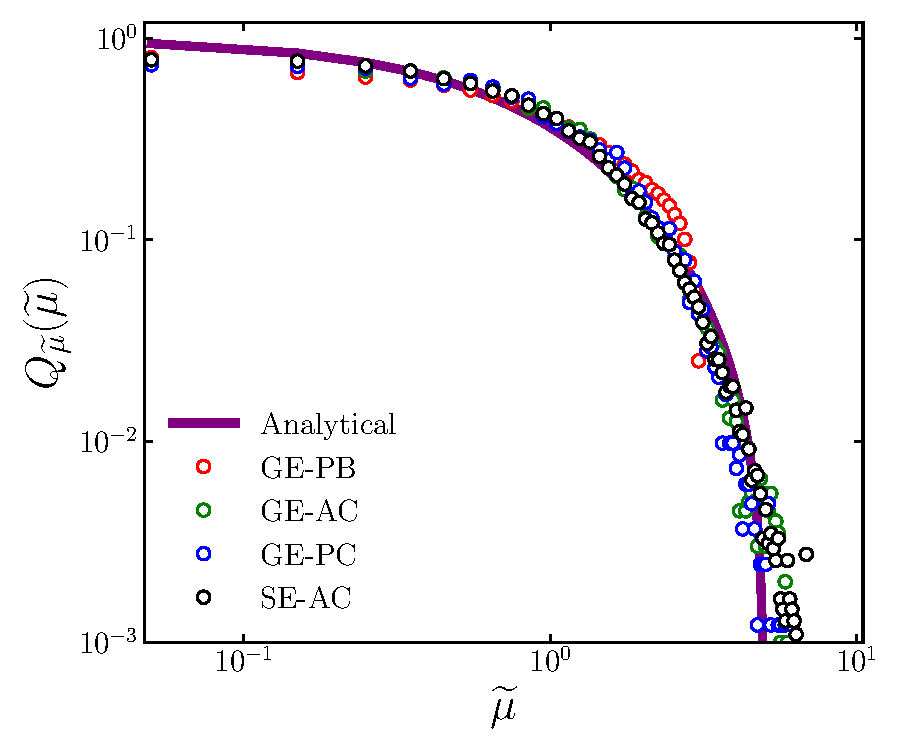
\includegraphics[width=0.8\linewidth]{chapters/chapter6/fig_4.pdf}
%     \caption{Scaled specific margin distributions $F(x)$ for multiple countries. While most countries (blue lines) follow the universal curve predicted by the RVM (black line), Ethiopia and Belarus (red lines) show significant deviations, suggesting potential electoral irregularities.}
%     \label{fig:anomalies}
% \end{figure}

\subsection{Case Studies: Electoral Anomalies}

Our analysis revealed two countries with pronounced deviations from the universal pattern: Ethiopia and Belarus. These deviations are significant enough to suggest potential irregularities in their electoral processes.

\subsubsection{The Ethiopia Case}

Ethiopia's 2010 election shows a striking deviation from the universal pattern, with the distribution of specific margins heavily skewed toward large values. This pattern indicates unusually large victory margins relative to turnout across the country's electoral units.

This statistical anomaly aligns with independent assessments of the 2010 Ethiopian election, which raised concerns about a restrictive political environment, uneven playing field, and potential irregularities in vote counting. The Ethiopia case demonstrates how the RVM can identify statistical signatures of electoral anomalies that correspond to documented concerns about electoral integrity.

\subsubsection{The Belarus Case}

Belarus similarly shows significant deviations from the universal pattern, with an overrepresentation of large specific margins. This statistical profile is consistent with concerns raised by international observers about Belarus's electoral processes, particularly regarding vote counting and tabulation.

The RVM's identification of statistical anomalies in both Ethiopia and Belarus demonstrates its value as an objective, quantitative tool for flagging potential concerns about electoral integrity. Importantly, these statistical indicators emerged purely from numerical analysis, without incorporating any qualitative assessments or contextual information about the countries' political systems.

\subsection{The RVM as a Statistical Baseline}

Beyond identifying potential irregularities, the RVM serves as a statistical baseline for understanding what "normal" electoral competition should look like. This baseline function has several valuable applications for election monitoring, historical analysis, cross-national comparison, and early warning of emerging concerns.

The RVM provides quantitative metrics to complement traditional monitoring approaches, allowing for standardized comparisons across different electoral systems. It can track the evolution of electoral competition over time, identifying shifts in statistical patterns that may indicate changes in the competitive environment. And it can serve as an early warning system, flagging unusual patterns that merit closer investigation by election observers and analysts.

\section{Limitations and Complementary Approaches}

While both the random nudge and the RVM provide valuable tools for addressing challenges to democratic processes, they have important limitations and should be viewed as complementary to other approaches rather than standalone solutions.

The random nudge approach cannot address structural causes of polarization such as economic inequality or institutional factors. Its effectiveness depends on implementation details and platform cooperation, and different cultural and political contexts may require different calibration. It may also be less effective against deliberate disinformation campaigns.

Similarly, the RVM diagnostic approach can identify statistical anomalies but cannot determine their causes. Some legitimate electoral systems may produce distributions that deviate from the universal pattern, and data quality issues can affect analysis results. Statistical signals must be interpreted in context alongside other evidence.

Both interventions are most effective when integrated with existing frameworks. The random nudge should complement media literacy programs, platform design improvements, and policy approaches to polarization. The RVM diagnostic tool should support, not replace, traditional election monitoring, legal frameworks, and institutional safeguards for electoral integrity.

\section{Implementation Pathways and Future Directions}

The translation of these theoretical tools into practical applications requires collaboration across multiple domains. For the random nudge, this includes conducting controlled trials to validate effectiveness and optimize parameters, forming partnerships with social media companies to implement and evaluate interventions, developing adaptive systems that learn and adjust intervention parameters based on observed effects, and incorporating user feedback and preferences into the design.

For the RVM diagnostic, implementation pathways include developing accessible software implementing RVM analysis for election observers and researchers, expanding data collection efforts to create more comprehensive and standardized electoral data, integrating statistical diagnostics into standard monitoring protocols, and training election officials and observers in statistical approaches to electoral integrity.

\section{From Research to Impact: The Path Forward}

Both applications—the random nudge for depolarization and the RVM for electoral diagnostics—represent promising pathways from fundamental research to real-world impact. Their development demonstrates how insights from statistical physics, complex systems, and computational social science can generate practical tools for strengthening democratic processes.

The ultimate success of these applications will depend on multidisciplinary collaboration, thoughtful implementation, and continuing refinement based on real-world experience. As we move forward, both approaches should be subject to rigorous validation, ethical scrutiny, and adaptation to diverse contexts.

In the concluding chapter, we will reflect on the broader implications of our research for understanding democratic processes and consider how the constructive use of randomness might inform other approaches to social system design and intervention. 